% !TeX root = report.tex
\documentclass[a4paper,11pt,dvipdfmx]{jsreport}

\usepackage{graphicx}
\graphicspath{{./images}{../images}}
\usepackage{pdfpages}
\usepackage{tikz}
\usepackage{xcolor}
\definecolor{UD_GREEN}{HTML}{03af7a}
\usepackage{bm}
\usepackage[left=30truemm]{geometry}
\usepackage{amsmath,amssymb}
\usepackage{docmute}
\usepackage{url}

\begin{document}


\tableofcontents

% 01.tex
\documentclass[platex,dvipdfmx]{jsreport}


\begin{document}
% \subfiletrue
\chapter{序論}


\section{背景}

  %% 目次
\subsection{フォトニック結晶}


フォトニック結晶は、1987年に、E.Yablonovitchが提案した概念であり、屈折率の異なる材質を周期的に配置した誘電体である。特に、フォトニックバンドギャップと呼ばれる、波数ベクトルに関わらず結晶中にどのモードも存在できないような周波数ギャップを持つように設計されたフォトニック結晶は、特定の方向への光の伝播を制御することが可能となる。
完全なフォトニックバンドギャップを有する構造には、一次元では多層膜、二次元では三角格子、三次元ではダイヤモンド構造などが知られている。


\subsection{MIT Photonic Bands}

MIT Photonic Bands (MPB) は、マサチューセッツ工科大学のSteven G. Johnsonによって開発された、ソフトウェアパッケージである。周期的誘電体構造における固有状態やバンド構造などの計算の機能を持っており、フォトニック結晶の研究に適している。また、フォトニック結晶に限らず、導波路や共振器システムなどの光学分野において活用することができる。

MPBは、誘電体構造の計算には時間領域法ではなく周波数領域法を用いている。これによって周波数と電磁モードを同時に取得を可能としている。従来の周波数領域固有ソルバーでは、目的の固有状態まで多数のバンドを計算する必要があったが、ターゲット固有ソルバーという手法を用いることでバンドギャップを直接解決し計算量と記憶容量のコストの削減を図っている。


技術的には、PythonやSchemeといった汎用のプログラミング言語から制御できるほか、HDF5形式での電場状態の出力に対応しているなど、他のプログラムと入出力において互換性を持たせるように設計された。libctl(Steven G. Johnsonによる開発)によって柔軟なインターフェースが提供され、手軽に条件を指定して計算することができる。またフーリエ変換にはFFTW (こちらもSteven G. Johnsonらによる開発)を用いている。現在もMITライセンスの元でオープンソースでメンテナンスされている。


\section{目的}
本研究では、フォトニック結晶の基礎的な構造である3次元フォトニック結晶に着目し、フォトニックバンドギャップが生じる構造の条件をMPBを用いて検証を行う。プログラムによって半径を連続的に変化させ、パラメータとバンドギャップの関連性を調べる。
本研究では、フォトニック結晶の構造の1つであるInverse Opals構造に着目して様々な条件下におけるバンドギャップの検証を行う。検証は、MPBを用いて行う。





\end{document}

%% 02.tex
\documentclass[platex,dvipdfmx,draft]{jsreport}

\usepackage{graphicx}
\graphicspath{{./images}{../images}}
\usepackage{pdfpages}
\usepackage{tikz}
\usepackage{xcolor}
\definecolor{UD_GREEN}{HTML}{03af7a}
\usepackage{bm}
\usepackage[left=30truemm]{geometry}
\usepackage{amsmath,amssymb}
\numberwithin{equation}{section}

\begin{document}

\chapter{原理}
\section{Maxwell方程式}
フォトニック結晶における電磁波の振る舞いは、Maxwell方程式によって記述される。Maxwell方程式は以下のように表される。
\begin{align}
  \nabla \times \bm{E} &= -\frac{\partial \bm{B}}{\partial t} \\
  \nabla \times \bm{H} &= \bm{j} + \frac{\partial \bm{D}}{\partial t} \\
  \nabla \cdot \bm{D} &= \rho \\
  \nabla \cdot \bm{B} &= 0
\end{align}

今回は、自由電荷や電流のない均一な誘電物質の混合誘電媒体を考えるため、$\rho = 0$、$\bm{j} = 0$となる。また、低損失の誘電体において、$\bm{D} = \epsilon(r) \bm{E}(\bm{r})$、透過率$\mu = 1$とみなすことで$\bm{B}(\bm{r}) = \mu \bm{H}(\bm{r}) = \bm{H}(\bm{r})$となる。

一般に、$\bm{E}$と$\bm{H}$は時間空間における複雑な関数であるが、Maxwell方程式は線形であることから、$\bm{E}$と$\bm{H}$を時間と空間の関数に分離することができる。すなわち、$\bm{E}(\bm{r},t) = \bm{E}(\bm{r}) e^{-i\omega t}$、$\bm{H}(\bm{r},t) = \bm{H}(\bm{r}) e^{-i\omega t}$とすることができ、Maxwell方程式は以下のように表される。
\begin{align}
  \nabla \cdot \bm{H}(\bm{r}) &= 0 \\
  \nabla \cdot \bm{D}(\bm{r}) &= 0 \\
  \label{eq:curlE}
  \nabla \times \bm{E}(\bm{r}) &= - \frac{i \omega}{c} \bm{H}(\bm{r}) \\
  \label{eq:curlH}
  \nabla \times \bm{H} (\bm{r}) &= \frac{i \omega}{c} \epsilon(\bm{r}) \bm{E}(\bm{r})
\end{align}

式(\ref{eq:curlE})と式(\ref{eq:curlH})より$\bm{E}(\bm{r})$を消去して、$\bm{H}(\bm{r})$についての式に整理すると以下のマスター方程式を得ることができる。
\begin{align}
  \label{eq:master}
  \nabla \times \left( \frac{1}{\epsilon (\bm{e})} \nabla \times \bm{H}(\bm{r}) \right) = \left( \frac{\omega}{c} \right)^2 \bm{H}(\bm{r}) 
\end{align}

式(\ref{eq:master})を固有値問題とするために、左辺の$\bm{H}(\bm{r})$に作用する演算子$\hat{\Theta}$を定義する。演算子$\hat{\Theta}$は回転を取り、$\epsilon(\bm{r})$で割って再度回転を取る微分演算子である。

次に、2つのベクトル場$\bm{F}$と$\bm{G}$について内積を以下のように定義する。
\begin{align}
  (\bm{F}, \bm{G}) = \int d\bm{r} \bm{F}^*(\bm{r}) \cdot \bm{G}(\bm{r})
\end{align}

このとき、演算子$\hat{\Theta}$は、任意のベクトル場$\bm{F}, \bm{G}$に対して次の内積関係が成立する。
\begin{align}
  \label{eq:inner}
  (\bm{F}, \hat{\Theta} \bm{G}) = (\hat{\Theta} \bm{F}, \bm{G})
\end{align}

式(\ref{eq:inner})は、演算子$\hat{\Theta}$がエルミート演算子であることを示しており、これはマスター方程式(\ref{eq:master})を解くときに得られる固有値が実数になりうことや固有値が異なる固有関数は互いに直行することなど、量子力学のシュレディンガー方程式と類似している。

マスター方程式(\ref{eq:master})にBlochの定理を適用すると、マスター方程式の解は次のように表される。
\begin{align}
  \bm{H}_{\bm{k}}(\bm{r}) = e^{i \bm{k} \cdot \bm{r}} \bm{u}_{\bm{k}}(\bm{r}) = e^{i \bm{k} \cdot \bm{r}} \bm{u}_{\bm{k}}(\bm{r + R})
\end{align}
ここで、$\bm{k}$はブロッホ波ベクトル、$\bm{R}$は格子ベクトルである。

\section{逆オパール(Inverse Opals)構造}
逆オパール構造は、フォトニック結晶の構造の1つである。Inverse Opals構造は、球状の粒子を三次元的に配置した構造であり、図\ref{fig:inverse_opals}のように、球状の粒子の間隔を空洞とし、空洞の中に誘電体を充填した構造である。
\begin{figure}[htbp]
  \centering
  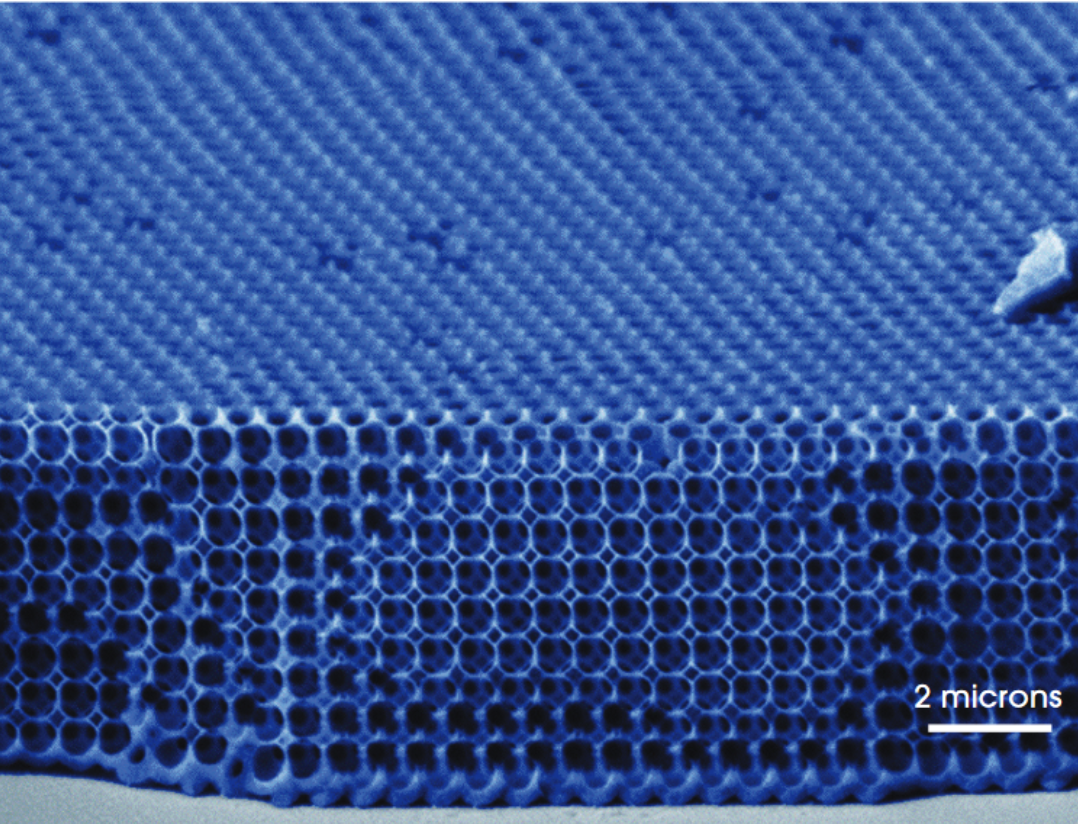
\includegraphics[width=0.6\linewidth]{inv_opals.png}
  \caption{逆オパール構造の電子顕微鏡像 \cite{text} p.103 より引用}
  \label{fig:inverse_opals}

\end{figure}

微細な球体を懸濁させたコロイドを蒸発させることによりfcc格子に自己集合させることができるので合成オパールは容易に製造することができる。合成オパールの球間に高誘電体物質を浸透させ、球を溶解させることで構造を反転させ、空気穴の逆オパールを作製することができる。

\section{ウッドパイル構造}
ウッドパイル構造は、棒状の誘電体物質を直行する方向に交互に積み重ねたものである。誘電体は丸太のような形状もあれば長方形の場合もある。
\begin{figure}[htbp]
  \centering
  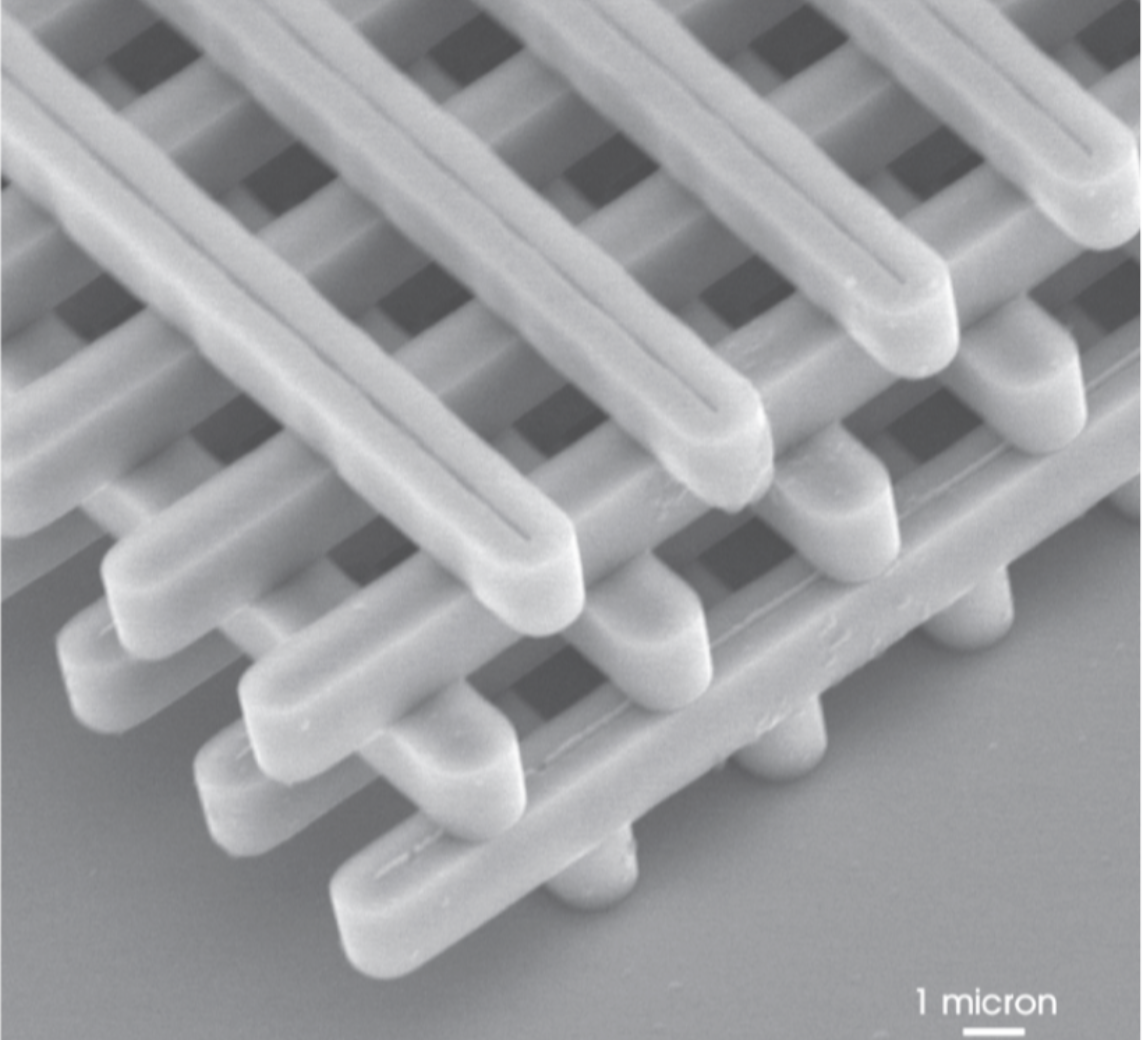
\includegraphics[width=0.6\linewidth]{woodpile.png}
  \caption{ウッドパイルフォトニック結晶の電子顕微鏡像 \cite{text} p.102 より引用}
  \label{fig:woodpile}

\end{figure}
最も単純に直行する方向に交互に積み重ねたものは、図\ref{fig:woodpile}のように、直方体の誘電体を交互に積み重ねたものである。この構造の場合、大きなギャップは生じない。より大きなギャップを生じさせるためには、ある方向を向いた層Aとそれに直交する方向の層Bに対して、それぞれ水平方向に半分だけずらした層C、Dを用いてABCDABCD$\cdots$のように並べることが有効である。

\section{ヤブロノバイト構造}
ヤブロノバイト構造は、図\ref{fig:yablonovite}のような構造をしており、発見者であるEli Yablonovitchらにちなんで名付けられた結晶構造である。誘電体のスラブ(板状の素材)に三角形配列の穴を開け、それぞれの穴を特定の角度で複数回(通常は三回)掘ることによって形成される。

\begin{figure}[htbp]
  \centering
  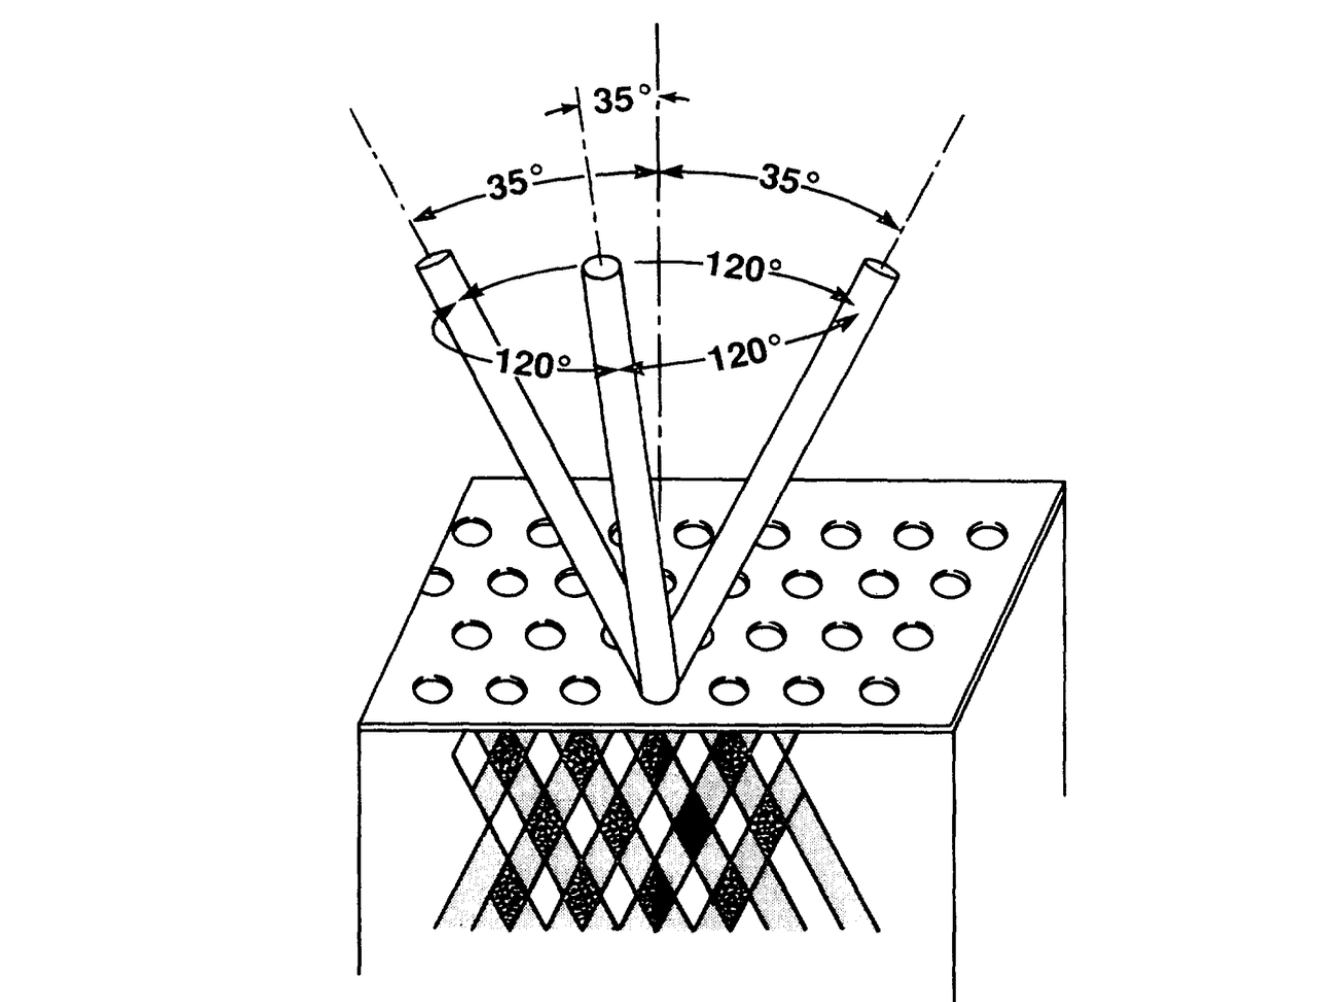
\includegraphics[width=0.6\linewidth]{yablonovite.png}
  \caption{ヤブロノバイト構造 \cite{orig}より引用}
  \label{fig:yablonovite}

\end{figure}


\section{2次元結晶の積み重ね}
\begin{figure}[htbp]
  \centering
  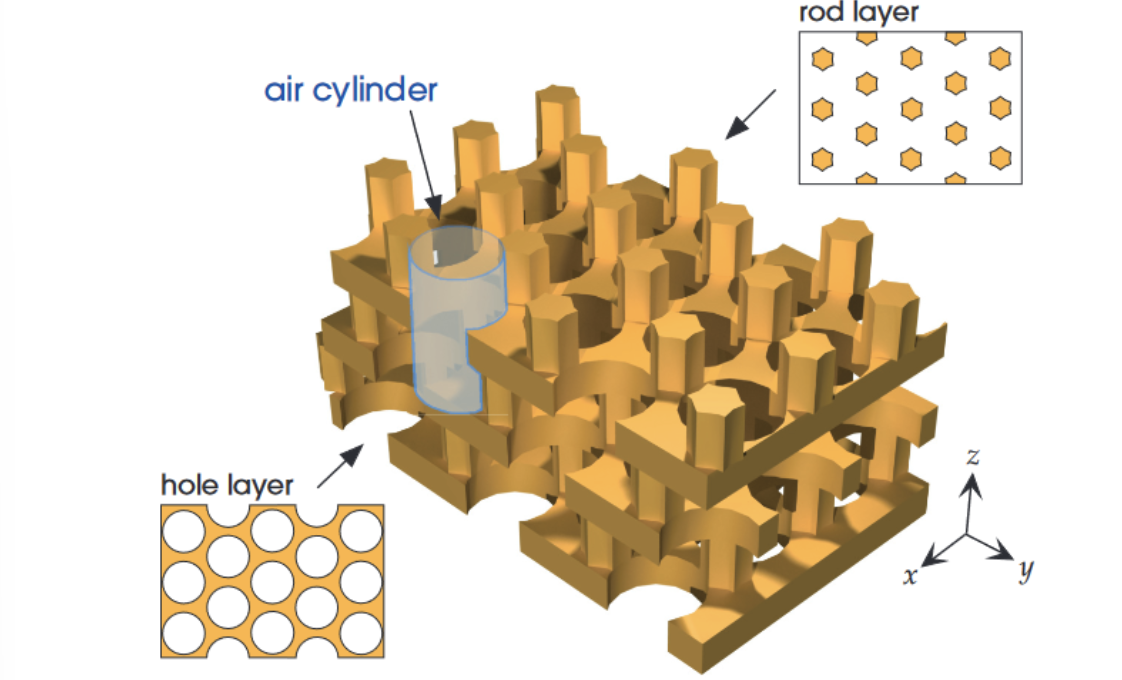
\includegraphics[width=0.6\linewidth]{2d.png}
  \caption{2次元結晶の積み重ねによる3次元結晶の作製 \cite{text} p.106 より引用}
  \label{fig:2d_3d}
\end{figure}
2次元結晶の積み重ねによって3次元結晶を作製することができる。

この結晶は空気中の高誘電体ロッドを三角格子状に並べたロッド層と、高誘電体中に円筒状の空気孔を三角格子状に並べたホール層により構成されている。

\section{ギャップ-ミッドギャップ比}
マスター方程式\ref{eq:master}において、$\epsilon(r)$を拡大または縮小した$\epsilon'(r)$を考える。このとき、$\epsilon'(r) = \epsilon(r / s)$であり、尺度に関するパラメータ$s$を用いて表すことができる。$r' = sr$、$\nabla' = \nabla / s$と変数変換を行うと、式\ref{eq:master}は以下のように表される。

\begin{align}
  s \nabla' \times \left( \frac{1}{\epsilon(\bm{r}'/s)} s \nabla' \times \bm{H}(\bm{r}'/s) \right)
  = \left( \frac{\omega}{c} \right)^2 \bm{H}(\bm{r}'/s)
\end{align}

$\epsilon(r' / s) = \epsilon' (r')$であることに注意して両辺を$s$で割ると、
\begin{equation}
  \begin{split}
  \nabla' \times \left( \frac{1}{\epsilon'(\bm{r}')} \nabla' \times \bm{H}(\bm{r}' / s) \right) =& \left( \frac{\omega}{cs} \right)^2  \bm{H}(\bm{r}' / s)
  \\
  =& \left( \frac{\omega'}{c} \right)^2 \bm{H}(\bm{r}' / s)
\end{split}
\end{equation}
これは、モードプロファイル$\bm{H}'(\bm{r}') = \bm{H}(\bm{r}' / s)$、周波数$\omega' = \omega / s$に関するマスター方程式である。

ここである結晶を係数$s$だけ拡大したときを考える。このとき、対応する周波数$\omega$は$1 / s$倍になる。
このとき、ギャップの中間部の周波数$\omega_m$とバンドギャップ幅$\Delta \omega$の比をギャップ-ミッドギャップ比と呼ぶ。ギャップ-ミッドギャップ比は、$\Delta \omega / \omega_m$で表される。以下に示す通りギャップ-ミッドギャップ比結晶のスケールに依存しない有用な評価手法である。

\begin{align*}
  \frac{\Delta \omega}{\omega_m} 
  = \cfrac{\cfrac{\omega_{\mathrm{max}}}{s} - \cfrac{\omega_{\mathrm{min}}}{s}}{\cfrac{\cfrac{\omega_{\mathrm{max}}}{s} + \cfrac{\omega_{\mathrm{min}}}{s}}{2}} 
  = \cfrac{\omega_{\mathrm{max}} - \omega_{\mathrm{min}}}{\cfrac{\omega_{\mathrm{max}} + \omega_{\mathrm{min}}}{2}}
\end{align*}

ここで、$\omega_{\mathrm{max}}$はバンドギャップの上端、$\omega_{\mathrm{min}}$はバンドギャップの下端における周波数である。

\end{document}
%% 03.tex
\documentclass[platex,dvipdfmx]{jsreport}



\begin{document}

\chapter{本論}

\end{document}
%% 04.tex
\documentclass[platex,dvipdfmx]{jsreport}

\usepackage{graphicx}
\graphicspath{{./images/}{../images/}}
\usepackage{pdfpages}
\usepackage{tikz}
\usepackage{xcolor}
\definecolor{UD_GREEN}{HTML}{03af7a}
\usepackage{bm}
\usepackage[left=30truemm]{geometry}
\usepackage{amsmath,amssymb}
\numberwithin{equation}{section}


\begin{document}

\chapter{結論}
すべての構造について言えることだが、結晶内の誘電体の誘電率が異なっていてもギャップの生じる範囲はあまり変わらずギャップマップの形状は非常に似通っていた。これを利用することで誘電率を細かく変化させたときにどこにギャップが生じるのか予想できる。



\end{document}

\chapter*{謝辞}
本研究に際し、フォトニック結晶の基礎をはじめとして様々なご指導をいただきました大淵泰司准教授、並びに貴重なご意見をいただいた大淵研究室の皆様に御礼申し上げます。



\begin{thebibliography}{2}
  \bibitem{orig} E.Yablonovitch, Phys.Rev.Lett.58, 2059(1987)
  \bibitem{text} John D. Joannopoulos, Steven G. Johnson, Joshua N. Winn, and Robert D. Meade, Photonic Crystals Molding the Flow of Light, PRINCETON, (1995).
  \bibitem{mpb} Massachusetts Institute of Technology, Steven G. Johnson,  MPB Documentation,
  \\ \url{https://mpb.readthedocs.io/en/latest/}  (参照2024-01-27).
  \bibitem{block} Steven G.Johnson and J.D.Joannopoulos, Block-iterative frequency-domain methods
  for Maxwell\'s equation in a planewave basis, OPTICS EXPRESS, Vol.8 No.3,173(2000)
  \bibitem{intro} David J.Griffiths, Introduction to Electrodynamics
\end{thebibliography}
\end{document}

